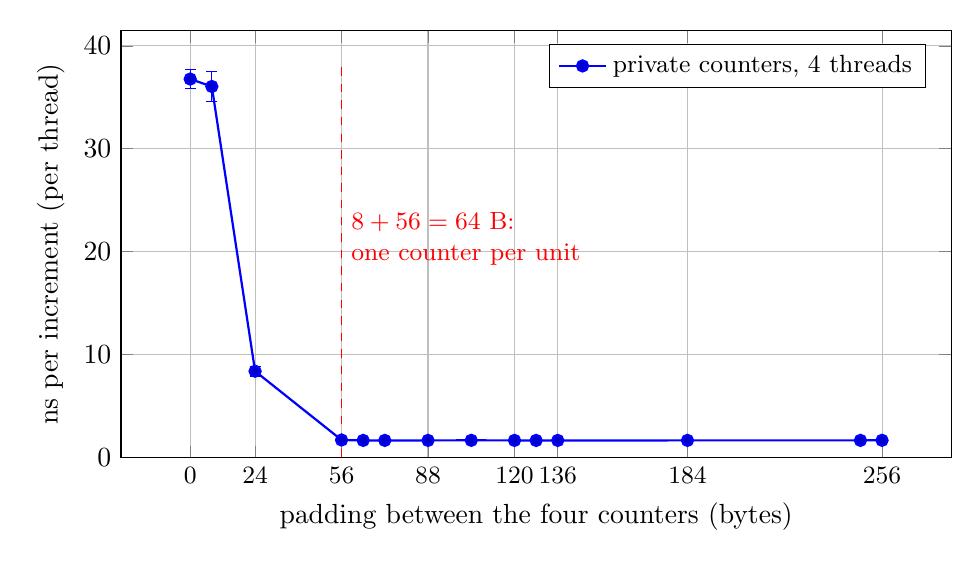
\begin{tikzpicture}
\begin{axis}[width=\textwidth, height=7cm, xlabel={padding between the four counters (bytes)}, ylabel={ns per increment (per thread)}, grid=major, ymin=0, xtick={0,24,56,88,120,136,184,256}, x tick label style={font=\small},
  legend pos=north east, legend style={font=\small}]
\addplot+[mark=*, thick, error bars/.cd, y dir=both, y explicit] coordinates {(0,36.771) +- (0,0.920) (8,36.046) +- (0,1.486) (24,8.381) +- (0,0.471) (56,1.693) +- (0,0.019) (64,1.655) +- (0,0.001) (72,1.655) +- (0,0.020) (88,1.655) +- (0,0.005) (104,1.661) +- (0,0.004) (120,1.655) +- (0,0.004) (128,1.651) +- (0,0.005) (136,1.652) +- (0,0.000) (184,1.656) +- (0,0.004) (248,1.657) +- (0,0.003) (256,1.663) +- (0,0.004)};
\addlegendentry{private counters, 4 threads}
\draw[dashed, red] (axis cs:56,0) -- (axis cs:56,38.61) node[pos=0.55, right, font=\small, align=left] {$8+56=64$ B:\\one counter per unit};
\end{axis}
\end{tikzpicture}